\documentclass[../main/main.tex]{subfiles}
\begin{document}

\chapter{Curvature}

%%%%%%%%%% LECTURE 8.III %%%%%%%%%%

\section{Curvature and gravity}
\textsf{Carroll, sec. 3.6}\\

The aim of this section is to give an answer to the following question: is there any \emph{intrinsic} way to characterize a ``honest''gravitational field? That is, a metric $g_{\mu\nu}(x)$ for which there does not exist any inertial frame $\hat x^\alpha$ in which
\[\de s^2=g_{\mu\nu}(x)\de x^\mu\de x^\nu=\eta_{\mu\nu}\de\hat x^\mu\de\hat x^\nu\qquad\text{and}\qquad\hchris\mu\rho\sigma\equiv0\]

Let us first observe that a property of Minkowski space is that the parallel transport between two points does not depend on the path. This is obvious in flat (inertial) coordinates, in which $\hchris\mu\rho\sigma\equiv0$
\[\cder{\hat V^\mu}\lambda\equiv\der{\hat V^\mu}\lambda=0\quad\Leftrightarrow\qquad\hat V^\mu(\lambda)=\text{constant}\]
which implies
\[\hat V^\mu_B\vert_{\gamma_1}=\hat V_A^\mu=\hat V^\mu_B\vert_{\gamma_2}\]
and
\[V^\mu_B\vert_{\gamma_1}= V^\mu_B\vert_{\gamma_2}\qquad\text{in any other coordinates }x^\mu\]
%
\begin{figure}[H]
\centering
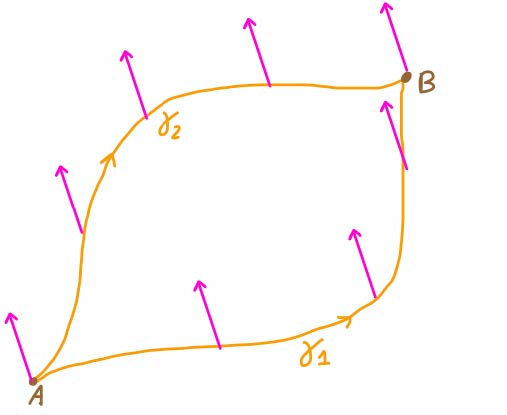
\includegraphics[width=6cm]{../img/curv-path-comm.jpg}
\end{figure}

For a more generic metric, we generally have $V^\mu(\lambda_{\text{fin}})\neq V^\mu(\lambda_{\text{in}})$. Indeed
\[\der{V^\mu(s)}s=-\chris\mu\nu\rho(X(s))V^\nu(s)\dot X^\rho(s)\]
which implies
\[V^\mu(s+\delta s)=V^\mu(s)=\chris\mu\nu\rho(X(s))V^\nu(s)\overbrace{\dot X^\rho(s)\delta s}^{\delta X^\rho(s)}+\dots\]
and then the infinitesimal change of $V^\mu$ parallely transported along $\delta X^\mu$ is given by
\[\delta V^\mu=-\chris\mu\nu\rho(x)V^\nu\delta X^\rho\]
%
\begin{figure}[H]
\centering
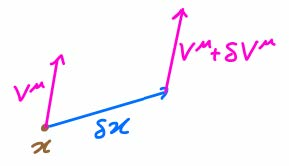
\includegraphics[width=4cm]{../img/curv-V-parall-trasp.jpg}
\end{figure}

Consider now two independent infinitesimal displacements $\delta_1X^\mu$, $\delta_2X^\mu$:
%
\begin{figure}[H]
\centering
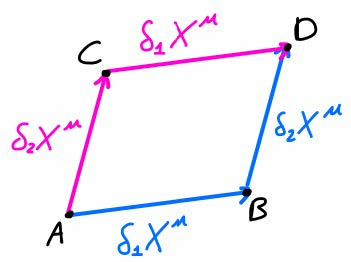
\includegraphics[width=5cm]{../img/curv-2-infinit-displ.jpg}
\end{figure}
in formulas we have (in the second step we used $x_B=x_A+\delta_1X$)
\begin{align*}
V_D^\mu\vert_{1-2}
&=V_B^\mu-\chris\mu\nu\rho(x_B)V_B^\nu\delta_2X^\rho\\
&=V_A^\mu-\chris\mu\nu\rho(x_A)V_A^\nu\delta_1X^\rho-\chris\mu\nu\rho(x_A)V_A^\nu\delta_2X^\rho\\
&\quad-\partial_\sigma\chris\mu\nu\rho(x_A)V_A^\nu\delta_1X^\sigma\delta_2X^\rho+\chris\mu\nu\rho(x_A)\chris\nu\alpha\sigma(x_A)V_A^\alpha\delta_1X^\sigma\delta_2X^\rho\\
V_D^\mu\vert_{2-1}&=(\text{the same with }1\leftrightarrow)
\end{align*}
Then $V_D^\mu\vert_{1-2}-V_D^\mu\vert_{2-1}=-\curv\mu\nu\rho\sigma(x_A)V_A^\nu\delta_1X^\rho\delta_2X^\sigma$ where we defined the \textbf{Riemann curvature}:
\begin{equation}\label{eqn:Riemann-curvature}\boxed{
\curv\mu\nu\rho\sigma\equiv\partial_\rho\chris\mu\nu\sigma-\partial_\sigma\chris\mu\nu\rho+\chris\mu\alpha\rho\chris\alpha\nu\sigma-\chris\mu\alpha\sigma\chris\alpha\nu\rho
}\end{equation}
Notice that this is a tensor. For any vector field $V^\mu(x)$ we have
\[[\nabla_\rho,\nabla_\sigma]V^\mu\equiv(\nabla_\rho\nabla_\sigma-\nabla_\sigma\nabla_\rho)V^\mu=\curv\mu\nu\rho\sigma V^\nu\]
(on the l.h.s. of the previous identity we omitted the factor $-\tens T\nu{\rho\sigma}\nabla_\nu V^\mu$ with $\tens T\nu{\rho\sigma}=2\Gamma^\nu_{[\rho\sigma]}$ since it vanishes). 

For more generic tensors $\tens T{\mu\dots}{\nu\dots}$ we have
\begin{align*}
[\nabla_\rho,\nabla_\sigma]\tens T{\mu\dots}{\nu\dots}
&=\curv\mu\tau\rho\sigma \tens T{\tau\dots}{\nu\dots}+(\text{similar action on \emph{upper} indices})\\
&\quad-\curv\tau\nu\rho\sigma \tens T{\mu\dots}{\tau\dots}+(\text{similar action on \emph{lower} indices})
\end{align*}
Note also that $[\nabla_\mu,\nabla_\nu]\phi=0$ for any scalar field. 

Note that for $\de s^2=\eta_{\alpha\beta}\de\hat x^\alpha\de\hat x^\beta$ we clearly have $\hcurv\mu\nu\rho\sigma\equiv0$, hence $\curv\mu\nu\rho\sigma\equiv0$ in any other coordinate system $x^\mu$ ( even if $\chris\mu\nu\rho\neq0$). Viceversa, if $\curv\mu\nu\rho\sigma\equiv0$ then one can find\footnote{See, for instance, Carroll pag. 124} a local coordinate system $\hat x^\alpha$ in which $\de s^2=\hat\eta_{\alpha\beta}\de\hat x^\alpha\de\hat x^\beta$. 

On the other hand, if $\curv\mu\nu\rho\sigma\not\equiv$ there do not exist inertial coordinates. Hence we arrived to the following important result:
\begin{equation}\boxed{\begin{split}
\text{spacetime is \emph{flat} (and locally like Mink)}\quad&\Leftrightarrow\quad\curv\mu\nu\rho\sigma\equiv0\\
\text{spacetime is \emph{curved}}\quad&\Leftrightarrow\quad\curv\mu\nu\rho\sigma\not\equiv0
\end{split}}\end{equation}

Note that (if $[x^\mu]=L$) the curvature has dimension $[\curv\mu\nu\rho\sigma]=(\text{length})^{-2}$. In particular, $(\curv\mu\nu\rho\sigma)^{-1/2}$ provides an estimate of the length scale $L$ above which the space-time cannot be approximated by the flat one. This also set the scale below which the EEP holds. 

Previous claim can be made precise by introducing \emph{normal} coordinates. 

\subsection{Geodesic (or Riemann) normal coordinates}

At any point $p$, choose orthonormal frame $e_\alpha=e_\alpha^\mu\partial_\mu$. Any $V\in T_pM$ can be decomposed as $V=\hat x^\alpha e_\alpha$
%
\begin{figure}[H]
\centering
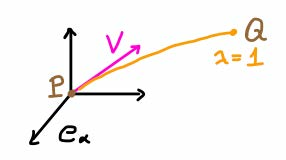
\includegraphics[width=4cm]{../img/curv-norm-coord.jpg}
\end{figure}
\noindent
Throw a geodesic with affine parameter $\lambda$ ($[\lambda]=1$) such that $\der{X^\mu}\de\lambda\vert_{\lambda=0}=V^\mu$. The value $\lambda-1$ identifies a point $q$, hence assign coordinates $\hat x^\alpha$ to $q$. In this way we obtained a defined coordinate system $\hat X^\alpha$ in a small enough neighbourhood of $\hat x^\alpha=0$. In this coordinate system
\begin{equation}\boxed{
\hchris\alpha\beta\gamma\vert_p=0\qquad\hat g_{\alpha\beta}(\hat x)=\eta_{\alpha\beta}-\frac13\hat R_{\alpha\gamma\beta\delta}\hat x^\gamma\hat x^\delta+\dots
}\end{equation}
and $\hat g_{\alpha\beta}=\eta_{\alpha\beta}+O\p{\frac{\hat x^2}{L^2}}$ with $L^2\simeq(\text{Riem})^{-2}$ as claimed above and $\hat x^2$ which approximates the proper ``distance'' from $p$. 

Such construction is the concrete realization of the EEP. The error is given by $\frac{(\text{distance})^2}{L^2}$ with $L^2\sim(\text{Riem})^{-1}$.

%%%%%%%%%%LECTURE 9%%%%%%%%%%%%%%%

\subsection{Properties of the Riemann tensor}

\textsf{Carroll, sec. 3.7}











\end{document}